\section{Auswertung}
\label{sec:Auswertung}

Die Maße, also Durchmesser $d$ bzw. Kantenlänge $a$ des eckigen Stabes mit quadratischem Querschnitt, Masse $m$ und Länge $l$ der Stäbe betragen

\begin{equation}
  a_{eckig} = 10,1 \pm 0,05mm \\
  m_{eckig} = 167,9 \pm 0,1g \\
  l_{eckig} = 620 \pm 0,05mm\\
\end{equation}

\begin{equation}
  d_{rund} = 10,1 \pm 0,05mm \\
  m_{rund} = 390,6 \pm 0,1g \\
  l_{rund} = 592 \pm 0,05mm \\
\end{equation}

Der eckige Stab besteht aus Aluminium, der runde aus Messing.\\
Die Literatiurwerte für die Elastizitätsmodule der Materialien lauten mit  nach 

\begin{equation}
  E_{Messing} =   \quad \textrm{und} \quad E_{Aluminium} = 
\end{equation}




\begin{figure}
  \centering
  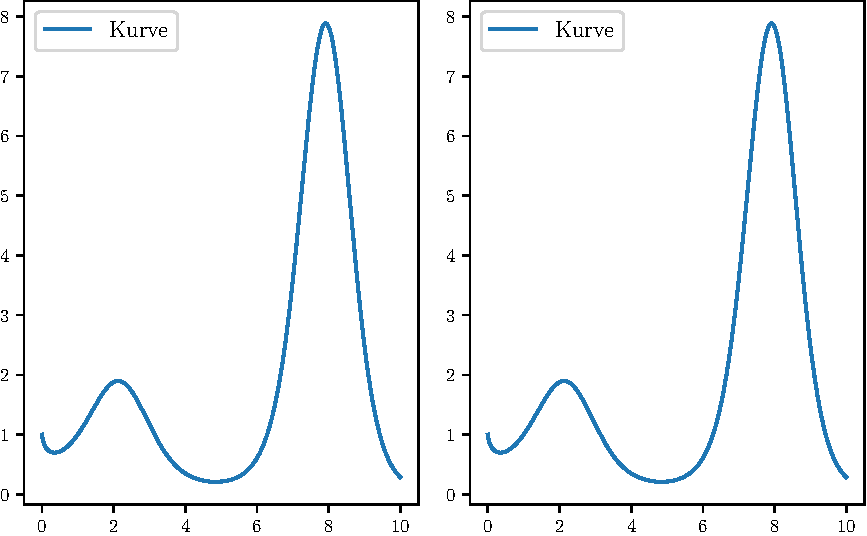
\includegraphics{plot.pdf}
  \caption{Plot.}
  \label{fig:plot}
\end{figure}


Siehe \autoref{fig:plot}! 
